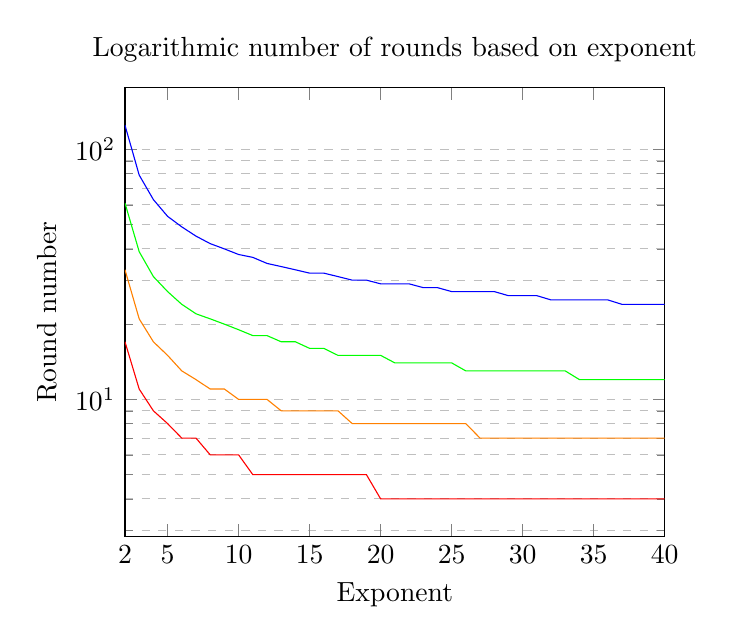
\begin{tikzpicture}
    \centering
    \begin{axis}[
        title={Logarithmic number of rounds based on exponent},
        xlabel={Exponent},
        ylabel={Round number},
        xmin=2, xmax=40,
        xtick={2,5,10,15,20,25,30,35,40},
        ytick={1,10,100},
        ymode=log,
        % legend pos=north east,
        ymajorgrids=true,
        yminorgrids=true,
        grid style=dashed,
    ]

    % REIKIA PATAISYT, KAD BUTU SCALE NUO 0, NES DABA NELEIDZIA NUO NULIO
    
    \addplot[color=red]
        coordinates {(2,17)(3,11)(4,9)(5,8)(6,7)(7,7)(8,6)(9,6)(10,6)(11,5)(12,5)(13,5)(14,5)(15,5)(16,5)(17,5)(18,5)(19,5)(20,4)(21,4)(22,4)(23,4)(24,4)(25,4)(26,4)(27,4)(28,4)(29,4)(30,4)(31,4)(32,4)(33,4)(34,4)(35,4)(36,4)(37,4)(38,4)(39,4)(40,4)};
        % \addlegendentry{Block size 17}
        
    \addplot[color=orange]
        coordinates {(2,33)(3,21)(4,17)(5,15)(6,13)(7,12)(8,11)(9,11)(10,10)(11,10)(12,10)(13,9)(14,9)(15,9)(16,9)(17,9)(18,8)(19,8)(20,8)(21,8)(22,8)(23,8)(24,8)(25,8)(26,8)(27,7)(28,7)(29,7)(30,7)(31,7)(32,7)(33,7)(34,7)(35,7)(36,7)(37,7)(38,7)(39,7)(40,7)};
        % \addlegendentry{Block size 33}

    \addplot[color=green]
        coordinates {(2,61)(3,39)(4,31)(5,27)(6,24)(7,22)(8,21)(9,20)(10,19)(11,18)(12,18)(13,17)(14,17)(15,16)(16,16)(17,15)(18,15)(19,15)(20,15)(21,14)(22,14)(23,14)(24,14)(25,14)(26,13)(27,13)(28,13)(29,13)(30,13)(31,13)(32,13)(33,13)(34,12)(35,12)(36,12)(37,12)(38,12)(39,12)(40,12)};
        % \addlegendentry{Block size 61}
        
    
    \addplot[color=blue]
        coordinates {(2,125)(3,79)(4,63)(5,54)(6,49)(7,45)(8,42)(9,40)(10,38)(11,37)(12,35)(13,34)(14,33)(15,32)(16,32)(17,31)(18,30)(19,30)(20,29)(21,29)(22,29)(23,28)(24,28)(25,27)(26,27)(27,27)(28,27)(29,26)(30,26)(31,26)(32,25)(33,25)(34,25)(35,25)(36,25)(37,24)(38,24)(39,24)(40,24)};
        % \addlegendentry{Block size 125}
        
    \end{axis}
\end{tikzpicture}